\documentclass[a4paper]{report}
\usepackage[utf8]{inputenc}
\usepackage[T1]{fontenc}
\usepackage{RJournal}
\usepackage{amsmath,amssymb,array}
\usepackage{booktabs}
\usepackage{hyperref}

\usepackage{Sweave}
\begin{document}

%% do not edit, for illustration only
\sectionhead{Contributed research article}
\volume{XX}
\volnumber{YY}
\year{20ZZ}
\month{AAAA}

%% replace RJtemplate with your article
\begin{article}
\Sconcordance{concordance:ephmetrics.tex:ephmetrics.rnw:%
1 8 1 1 0 20 1 1 6 13 1 1 2 1 0 1 1 16 0 1 2 1 1 1 4 7 0 1 2 2 1 1 2 1 %
0 1 1 13 0 1 2 19 1}


\title{Ephmetrics}
\author{Ben Morton}

\maketitle

%%\VignetteIndexEntry{Using the facage package}
%%\VignetteDepends{facage}


\abstract{The \pkg{ephmetrics} package analyzes Williams College Archived Course Catalogs in PDF form and reports specific data. This data includes information about the given year's tuition price, geographical distribution, and size of the undergradute classes}

\section{Introduction}


\section{Data}
The information in this package retrieves data from the Registrar Office of Williams College Archived Course Catalogs. These catalogs are found in PDF form, and the pdftools package was used to read and convert the PDF’s into text. Using the 2009-2010 catalog as a test case, functions were developed to capture the relevant information from the given year.

The format of the catalog from each year is not exactly uniform, so the functions require updating based on the assumptions that were made. Examples of this are column layouts, what specific data follows what, and the overall formatting of each year’s information.

\section{Examples of Using the Data}

\begin{Schunk}
\begin{Sinput}
> price_data <- ephmetrics::get_price_data()
> price_data
\end{Sinput}
\begin{Soutput}
   Tuition Year
1    46330 2014
2    44660 2013
3    42938 2012
4    41190 2011
5    39250 2010
6    37400 2009
7    35438 2008
8    33478 2007
9    31548 2006
10   29786 2005
\end{Soutput}
\end{Schunk}
\begin{Schunk}
\begin{Sinput}
> print(ggplot(price_data, aes(x = Year, y = Tuition)) +
+         geom_line() +
+         geom_point())
\end{Sinput}
\end{Schunk}
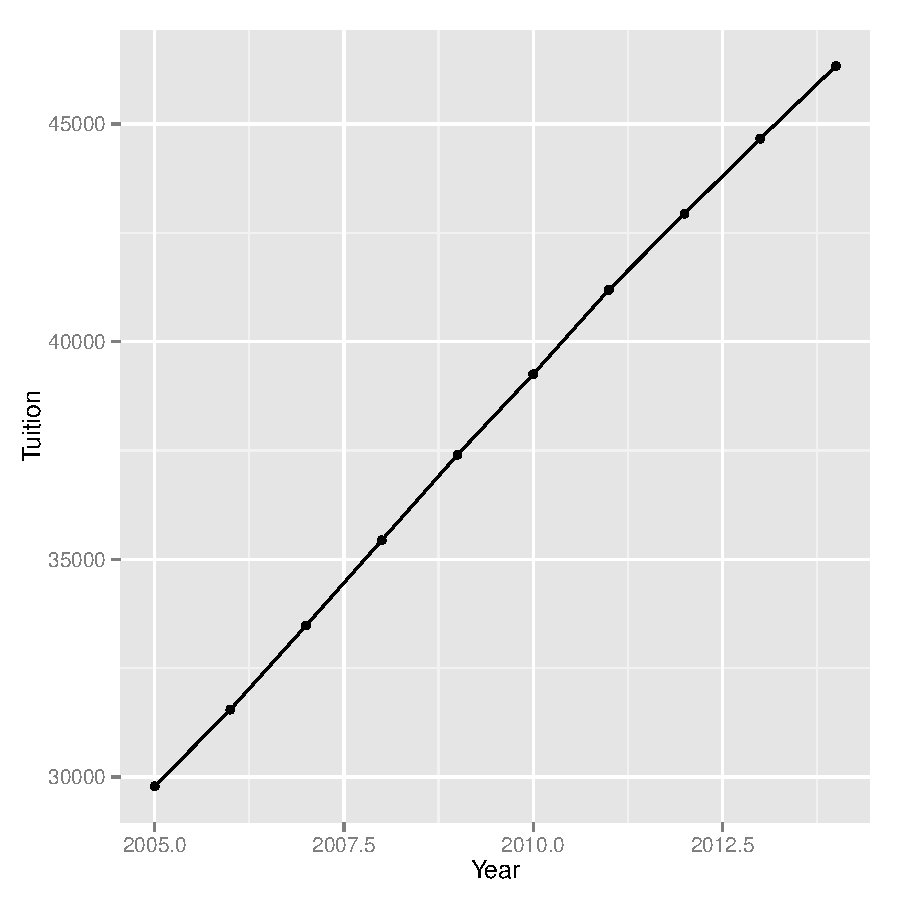
\includegraphics{ephmetrics-003}
\section{Conclusion}

\address{Ben Morton\\
  Mathematics and Computer Science\\
  Williams College\\
  Williamstown, MA, USA\\}
\email{bmm5@williams.edu}

\end{article}

\end{document}




